\chapter{System Architecture}
\label{chapter:architecture}

\textbf{Author: Lukas Leskovar} 

This chapter aims to provide a thorough overview of Autumns system architecture by describing its construction as well as logical and computational  structure. To this end, the difficulties faced during development and decisions made that affected the overall project are described.

\section{First Prototype}
The first version of the Autumn drone consisted of three main components:
\begin{itemize}
	\item A DJI Matrice 100 functioning as the base of the system powering all external components.
	\item To perform 3D mapping a Stereolabs ZED 1 was mounted onto the lower front part of the drone
	\item As the main component used to compute 3D mapping and control the drone a NVIDIA Jetson TX2 was mounted onto the drones expansion bay.
\end{itemize}
This prototype quickly demonstrated which part of the system needed to be improved where as the main issues were the lack of computational power and usage of non optimal hardware. A detailed explanation as well as a multitude of solutions to this problem are discussed in the following sections.


\section{Processing and power management}
%In the past decades the computational power of microprocessors has dramatically increased to the point where the transistors contained in these processors cannot be built smaller thus limiting the overall computational power.

%In the past decades research has pushed the limits of computational performance of processors further to its limits, all while performing a trade off concerning power requirements. Modern circuits can execute complex algorithms with high speed calculations but therefore have high energy requirements. 
%This confrontation of performance and power is a major issue faced in most robotic applications and therefore affected the implementation of this diploma thesis. In order to perform 3D mapping and local navigation, Autumn requires to execute complex and load heavy algorithms that will be discussed in further detail in later sections. 

In the past decades research has made vast improvements concerning the performance of processors whether they are used as stand-alone microprocessors, microcontrollers, embedded processors or digital signal processors. However these improvements come at the cost of higher power requirements. This trade-off is a major concern in many robotic applications that are powered by batteries or are restricted to low power inputs. Since Autumn is powered only by a drone battery this issue is groundbreaking during the development of this diploma thesis. 

The central component of the system is a NVIDIA Jetson TX2 board equipped with a 2GHz NVIDIA Denver2 dual-core and a 2GHz Arm Cortex-A57 quad-core processor. \footcite{jetsonHardwarePageNoDate}

Using NVIDIA tegrastats \footcite{nvidiaTegrastatsNoDate} the average power consumption of the system at an idle state was measured at 2.7W. However while performing non optimized 3D mapping and navigation algorithms (Chapter \ref{chapter:slam}) with both processors fully utilized and Max-N power mode activated the average power consumption reached 7.9W. \footcite{jetsonPowerModesNoDate} 
%schreib drüber dass diese zahlen bedeuten dass das system komplett ausgelaset ist
Operating the system at such high stress does not only quickly drain the drones battery but also impairs the quality of the resulting 3D map as well as operating the drone.


\section{Solving processing limitations}
When dealing with load heavy computations one way to solve quality issues is to use higher performance hardware, however due to aforementioned power constraints and drone payload requirements this approach is not suitable for this project. 
Another possible solution is to lower the computational load of the processors therefore improving result quality and lowering power consumption. 
This approach was tested in the following two forms:
\begin{itemize}
%	\item Distributing high power computations to a remote host. For most applications out- sourcing computation to a cloud would be the optimal solution however the work en- vironment of Autumn does not allow for a sufficient internet connection. The only possible way to implement this approach was to bring a powerful computer on site and have it wirelessly communicate with the Autumn drone.
	
	\item Distributing high power computations to a remote host. This approach loweres the amount of computation on the drone but requires to use a high performance computer on site to wirelessly communicate with the drone. Furthermore the wifi-range becomes another limiting factor since with increasing range the latency increased thus impairing the result quality again.
	
	\item The second approach was to disable visual odometry using feature extraction and pattern matching as the most complex part of the algorithm and providing odometry using a much more performant visual inertial odometry algorithm. To this end the drone was equipped with a Stereolabs ZED 2i stereo-camera which is benchmarked against other sensors in section \ref{chapter:sensors}%which performed a hardware accelerated sensor-fusion of Inertial Measurement Unit (IMU) Data and visual odometry. %Furthermore the overall mapping quality compared to the Stereolabs ZED 1 was improved due to better depth sensing technology. 
\end{itemize}

\section{Final Product}
\label{sec:finalProduct}
Following the aforementioned approach the main causes of performance issues where eliminated by replacing non optimized hardware components and distributing non-critical computations such as user interaction or path planning to a remote host as impairing these aspects of the system by latency would not pose less of a problem. 
With these adjustments the Autumn drones final version consisted of the following altered components:
\begin{itemize}
	\item As already mentioned the Stereolabs ZED 1 was replaced by its successor the Stereolabs ZED 2i. With its additional sensors and out of the box sensor fusion available it greatly reduced the amount of computations performed on the NVIDIA Jetson TX2. 
	\item In order to establish a connection to a remote host and perform computations the Dual Band 2.4GHz and 5GHz Antennas of the NVIDIA Jetson TX2 where utilized. 
	\item A laptop serving as the remote host was added to the system performing non-critical computations.
\end{itemize}

\begin{figure}
	\centering
	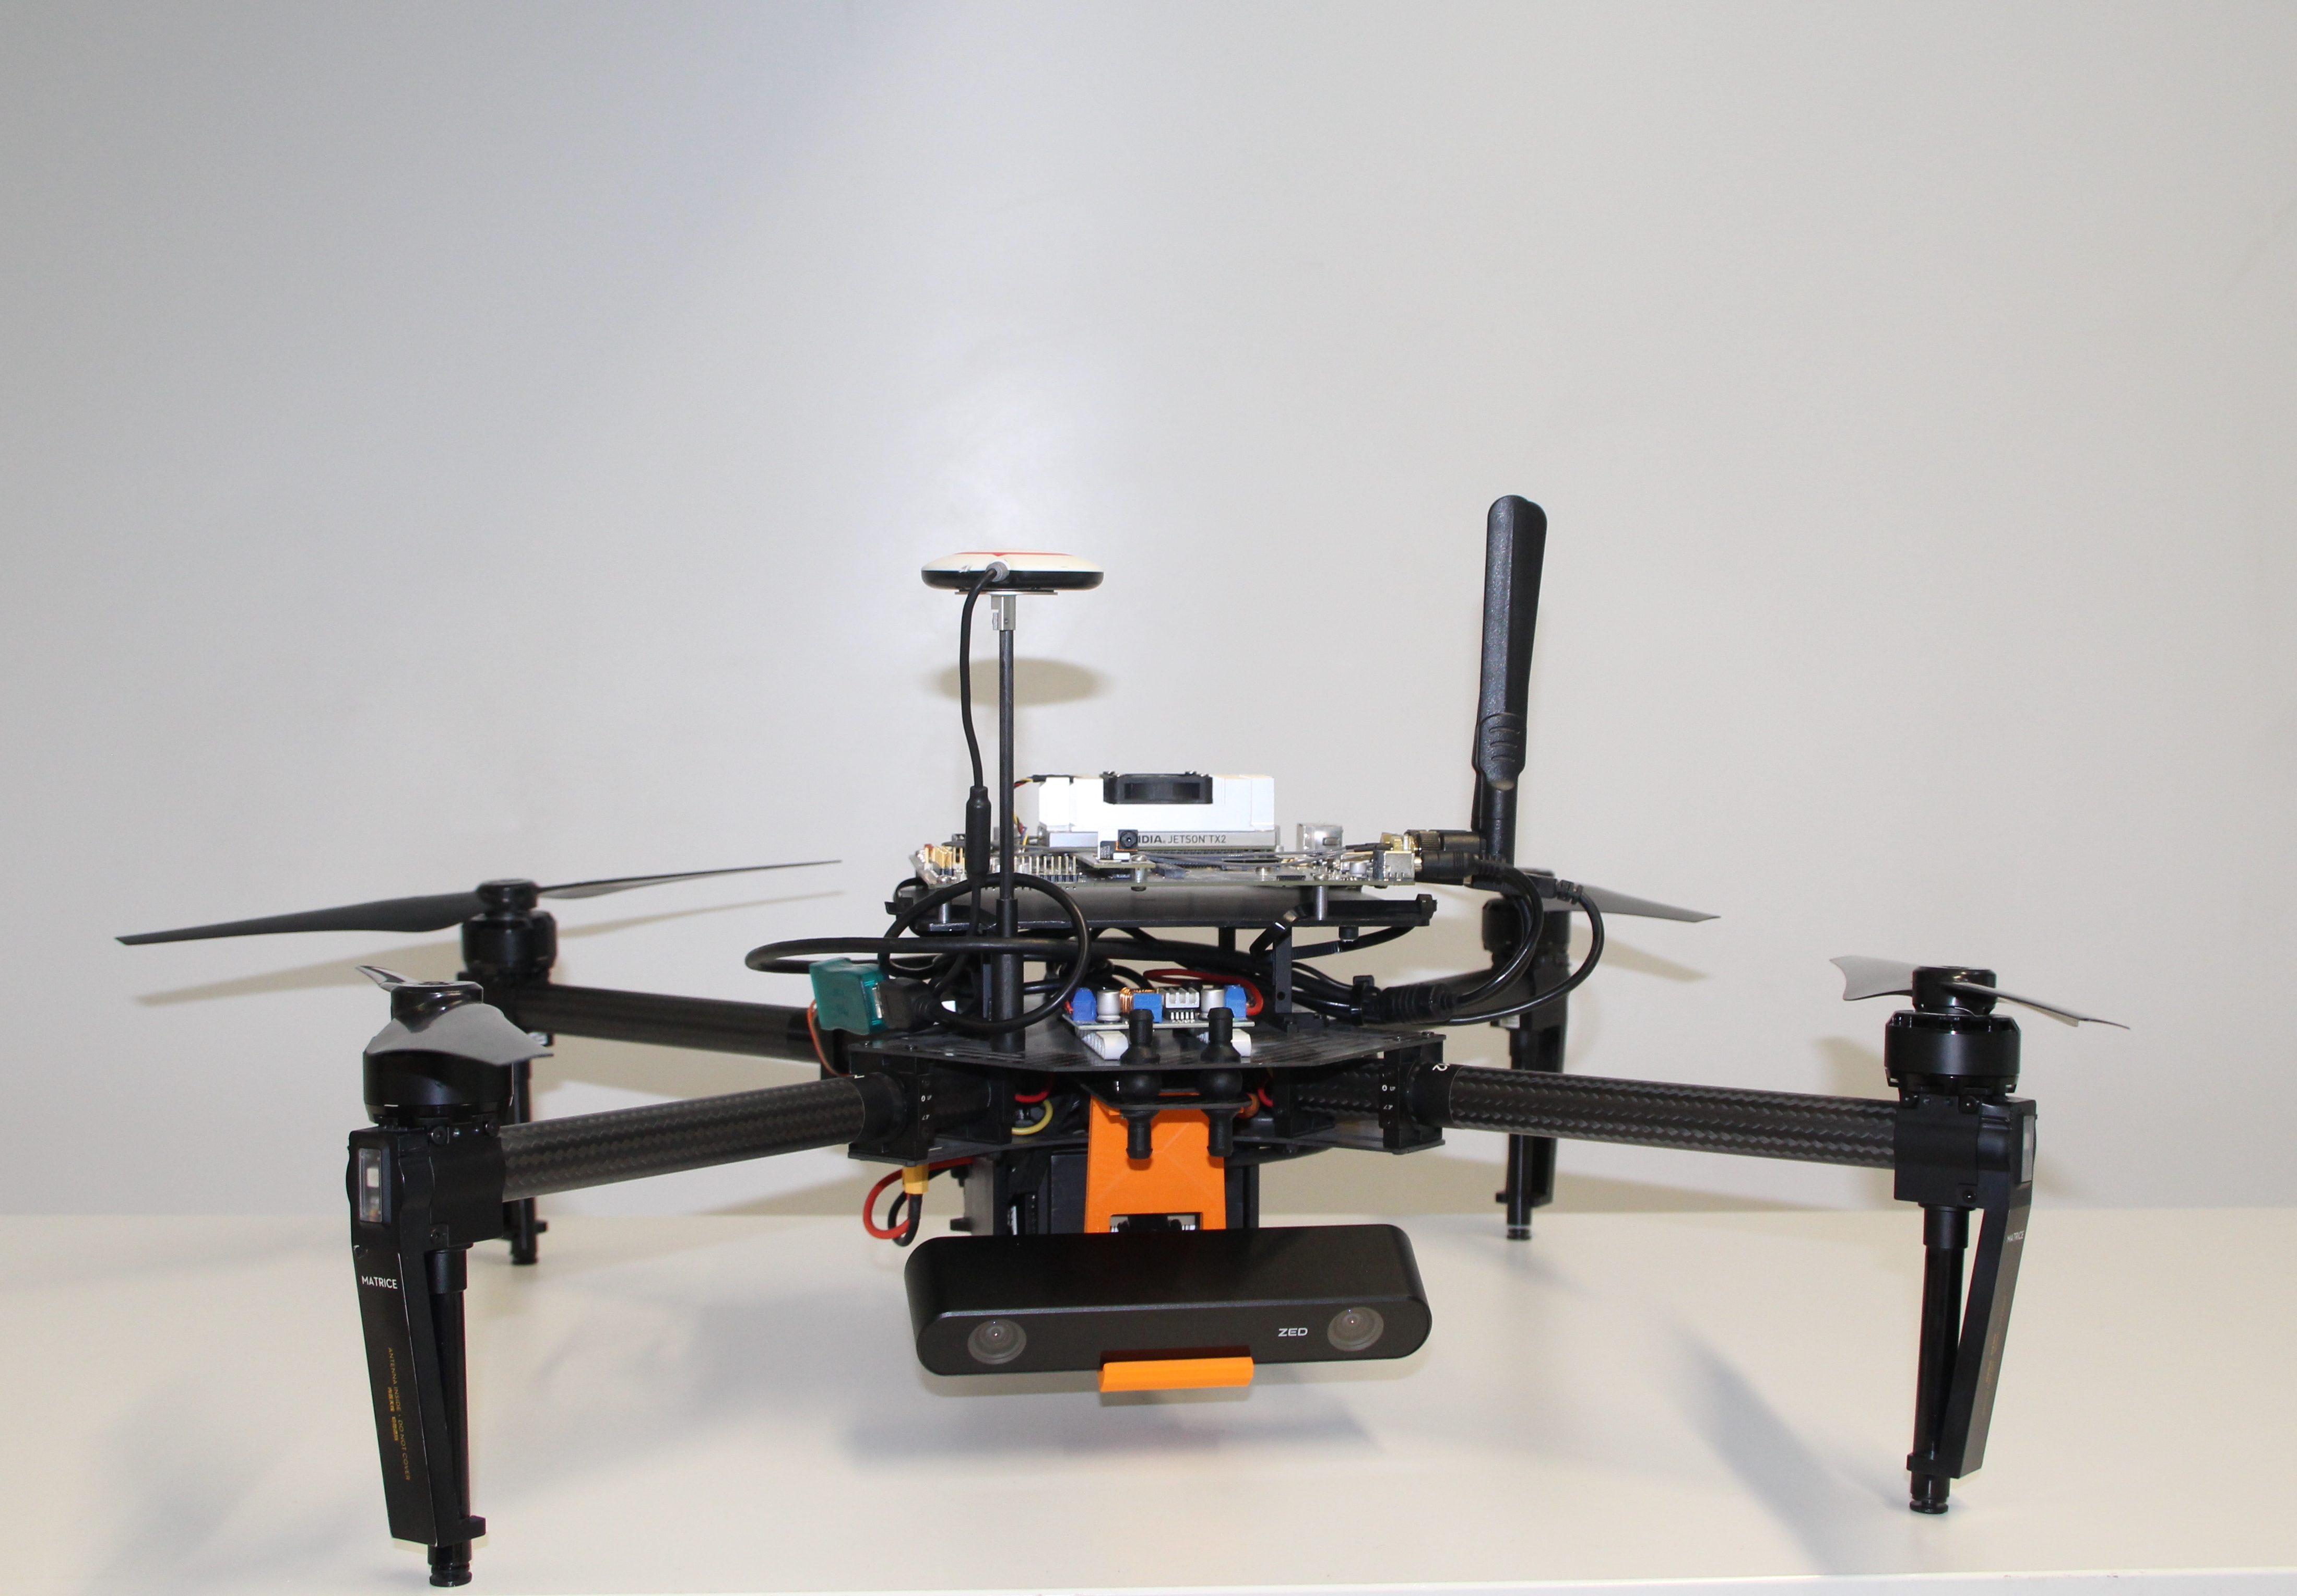
\includegraphics[width=0.9\linewidth]{img/autumnDrone}
	\caption{
		The Autumn drone with the NVIDIA Jetson TX2 on top as well as the Stereolabs ZED 2i mounted onto the drones Gimbal mounting plate using a custom 3D printed frame. 
	}
	\label{fig:autumn}
\end{figure}


\section{Autumn Lifecycle}
\textbf{Author: Fabian Kleinrad} 

This section is going to go in depth about how different modules in the autumn project interoperate. Hereby an overview will be given, that will illustrate how the autumn project works. The theoretical approach in this project is closely represented by the techniques explained in detail in section 
!!!UNCOMMENT!!!%\ref{autumnControlLoop}
. In contrast this section concerns itself with the practical realization of these concepts

\subsection{Lifecycle Modules}

Autumn contains four modules delimited from one another. Like the name suggests these fundamental building blocks of the project are modular. By that means, it is made possible to change or improve certain parts without the need to integrate the changes into all other aspects present in autumn.

\subsubsection{Drone} This component represents the physical drone and sensory equipment installed on the autumn drone, described in section \ref{sec:finalProduct}.  
\subsubsection{SLAM} The SLAM component converts the sensor data, provided from the drone into a digital representation. Chapter \ref{chapter:slam} goes into detail how this is realized.
\subsubsection{Navigation} The module navigation is used to plan routes through the abstracted environment explained in chapter \ref{chapter:abstract_env}.. Hereby the functionality of this module is divided into two components.
	\begin{itemize}
		\item Explorer - decides next waypoint
		\item Path-Planning - Plans path to new waypoint, explained in chapter \ref{chapter:path_planning}
	\end{itemize}
\subsubsection{Drone Control}
Drone control acts as the intermediary between the physical drone and virtual instruction stemming from the navigation component. Drone control can be realized autonomous or semi-autonomous. Semi-autonomous hereby refers to, the user providing flight instructions depended on the navigation output.

\subsection{Module cooperation}

From a process oriented standpoint the autumn lifecycle begins with the drone perceiving its environment. The data captured by the sensor equipment the drone is equipped, are stereo images and data from an inertial measurement unit. This data in succession allows an SLAM algorithm to perform its localization and mapping. Upon finishing SLAM provides a digital representation of the space the drone has been able to observe. These abstractions and how such a SLAM algorithm works are covered in chapter slam(\ref{chapter:slam}) and chapter abstract environments(\ref{chapter:abstract_env}). Using this representation of the environment, an path planning algorithm is used, along with an algorithm determining where the drone should move next. This choosing of the next waypoint is realized in autumn via the explorer. For autumn the user provides the point for the explorer. The final step in the navigation component is using the a path planning algorithm, described in chapter \ref{chapter:path_planning}, to calculate a path to the goal point. Based on this path drone control is able to send flight instructions using the dji-sdk to control the movements of the drone.

\begin{figure}[h]
	\centering
	\includesvg[width=.8\linewidth]{img/svg/AutumnLifeCycle}
	\caption{Depiction of the autumn lifecycle, with its four components and the communication between them}
	\label{fig:autumnLifecycle}
\end{figure}


\filbreak